\documentclass[aspectratio=1610,14pt,t]{beamer}

% Colors
\usepackage{color}
\definecolor{mainorange}{HTML}{EC811B}
\definecolor{lightgrey}{HTML}{888888}
\definecolor{almostwhite}{HTML}{FEFEFE}

% Syntax highlighting
\usepackage{minted}
\usepackage{alltt}
\newcommand\hi[1]{{\color{mainorange} \textbf{#1}}}

% Custom unicode symbols
\usepackage{newunicodechar}
\newcommand\Warning{%
 \makebox[1.4em][c]{%
 \makebox[0pt][c]{\raisebox{.1em}{\small!}}%
 \makebox[0pt][c]{\color{red}\Large$\bigtriangleup$}}}%

\newunicodechar{⚠}{\Warning}

% Theme
\usetheme[%
  subsectionpage=progressbar,
  numbering=fraction,
  progressbar=foot,
]{metropolis}

% Customization
\usepackage{pagecolor}
\setbeamertemplate{section in toc}[sections numbered]
\setbeamerfont{title}{size=\fontsize{30}{30}}
\setbeamerfont{block title}{size=\large}
\newcommand\sep{\textcolor{lightgrey}{\rule{\linewidth}{0.05mm}}}

% Positioning
% https://tex.stackexchange.com/a/34929/13059
\def\Put(#1,#2)#3{\leavevmode\makebox(0,0){\put(#1,#2){#3}}}

% Meta
\title{Embedded Rust}
\date{2018-01-30}
\author{Raphael Nestler (@rnestler)}
\institute{Rust Zürichsee Meetup}

\begin{document}

\pgfdeclareimage[width=\paperwidth]{bg}{background-dark.pdf}
\pagecolor{almostwhite}  % Prevent speakerdeck from optimizing away the bg color
\usebackgroundtemplate{\pgfuseimage{bg}}
\maketitle

% ----------------------------------------------------------------- %

\begin{frame}[c]{println!("{:?}", Self)}
  Hi! I'm Raphael (@rnestler).

  \pause I live in Rapperswil

  \pause I work at Sensirion ({\small \url{https://sensirion.com}}).

  \pause I'm a founding member of Coredump\\hackerspace ({\small \url{https://coredump.ch}}).
\end{frame}

% ----------------------------------------------------------------- %

\begin{frame}[plain,noframenumbering]
  \frametitle{Outline}
  \setcounter{tocdepth}{1}
  \tableofcontents
\end{frame}

% ----------------------------------------------------------------- %

\pgfdeclareimage[width=\paperwidth]{bg}{background-light.pdf}
\usebackgroundtemplate{\pgfuseimage{bg}}

\section{Embedded Programming}

\begin{frame}[c]{What is an \emph{Embedded System}?}
  \begin{quote}
    A combination of computer hardware and software, and perhaps
    additional mechanical or other parts, designed to perform a dedicated
    function.
  \end{quote}
  Michael Barr. ``Embedded Systems Glossary''\footnote{\tiny\url{https://barrgroup.com/Embedded-Systems/Glossary-E\#embedded\_system}}
\end{frame}

\begin{frame}[c]{What is embedded programming?}
  \begin{itemize}
    \item Dedicated, not general purpose, µC system
    \item<1-> Baremetal
    \item<1-> Low-Level
    \item<2-> For this talk: Bare metal on Cortex-M MCUs
  \end{itemize}
\end{frame}

\begin{frame}[c]{Why do they say it's hard?}
  \begin{itemize}
    \item Harsh environment (No OS which protects you)
    \item Resource constrained (Remember dedicated?)
    \item Non-standard, Non-OSS toolchain
    \item Hard realtime requirements
    \item \ldots
  \end{itemize}
\end{frame}

\begin{frame}[c]{Why could Rust be awesome for it?}
  \begin{itemize}
    \item Zero cost abstractions!
    \item Provides safety at compiler level, not OS
    \item Expressive type system to encode constraints
  \end{itemize}
\end{frame}

\section{Notable projects}

\begin{frame}[c]{\url{https://zinc.rs}}
  \begin{itemize}
      \item Proof-of-concept, currently abondoned
      \item Descripe system in a DSL (platformtree)
      \item Use macros to convert into setup code
      \item Promising concept!
  \end{itemize}
\end{frame}

\begin{frame}[c,fragile]{Platformtree}
  \begin{minted}[fontsize=\small]{rust}
platformtree!(
  // use lpc17xx
  lpc17xx@mcu {
    clock {
      // source is clocked from main (external) oscillator running at 12MHz
      source = "main-oscillator";
      source_frequency = 12_000_000;
      // configure pll to output 100MHz
      pll {
        m = 50;
        n = 3;
        divisor = 4;
      }
    }
  \end{minted}
\end{frame}

\begin{frame}[c,fragile]{Platformtree}
  \begin{minted}[fontsize=\small]{rust}
    timer {
      // define configuration for timer 1
      timer@1 {
        counter = 25;
        divisor = 4;
      }
    }
    gpio {
      // define pins for gpio port 1
      1 {
        // pins 18 and 20 are gpio out
        led1@18 { direction = "out"; }
        led2@20 { direction = "out"; }
      }
  \end{minted}
\end{frame}

\begin{frame}[c,fragile]{zinc.rs app code}
  \begin{minted}[fontsize=\small]{rust}
fn run(args: &pt::run_args) {
  // toggles pin values
  args.led1.set_high();
  args.led2.set_low();
  // wait for 1 second
  (args.timer as &zinc::hal::timer::Timer).wait(1);

  args.led1.set_low();
  args.led2.set_high();
  (args.timer as &zinc::hal::timer::Timer).wait(1);
}
  \end{minted}
\end{frame}

\begin{frame}[fragile]{Getting started with zinc.rs}
  \begin{minted}[fontsize=\small]{bash}
# Old nightly
rustup override set nightly-2016-09-17
# downgrade xargo
cargo install xargo --version 0.2.0 --force
# build and download
cd examples/blink_lpc17xx
xargo build --release --target thumbv7m-none-eabi
arm-none-eabi-objcopy -O binary\
  ./target/thumbv7m-none-eabi/release/blink blink.bin
cp blink.bin /run/media/roughl/MBED
  \end{minted}
\end{frame}

\begin{frame}[c]{zinc.rs demo time!}
\end{frame}

\begin{frame}[c]{\url{https://www.tockos.org/}}
  \centering
  
\includegraphics[width=.8\textwidth]{img/tock.png}

  \begin{quote}
    An embedded operating system designed for running multiple concurrent,
    mutually distrustful applications on low-memory and low-power
    microcontrollers.
  \end{quote}
\end{frame}

\begin{frame}[c]{tockos}
  \begin{itemize}
    \item Uses ``capsules'' for kernel component isolation
    \item Memory Protection Units (MPU) based isolation for processes
  \end{itemize}
\end{frame}

\begin{frame}[c]{xargo, svd2rust, cortex-m-quickstart}
  \begin{itemize}
    \item xargo\footnote{\url{https://github.com/japaric/xargo}}:
      The sysroot manager that lets you build and customize std

    \item svd2rust\footnote{\url{https://github.com/japaric/svd2rust}}:
      Generate Rust register maps (structs) from SVD files

    \item cortex-m-quickstart\footnote{\url{https://github.com/japaric/cortex-m-quickstart}}:
      A template for building applications for ARM Cortex-M microcontrollers
    \item<2-> Brought to you by the amazing japaric!
  \end{itemize}
\end{frame}

\section{Case study LPC11U24}

\begin{frame}[c]{water-sensor project}
  \centering
  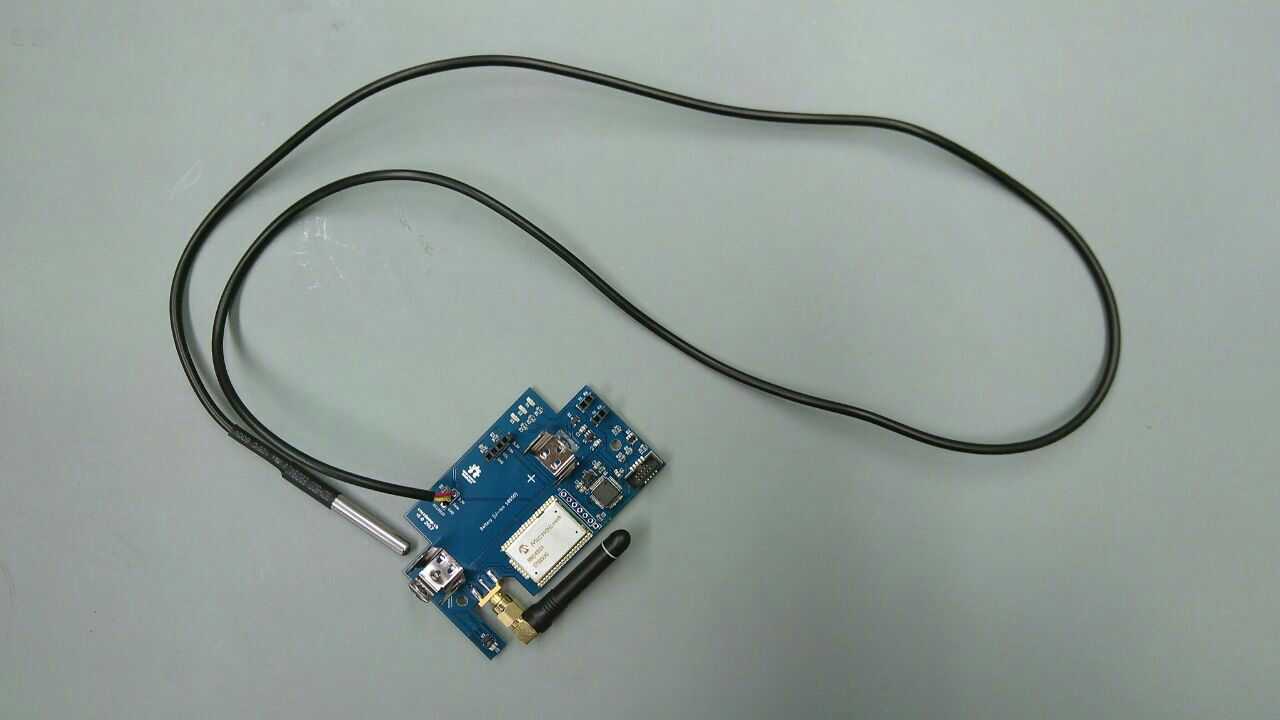
\includegraphics[width=.9\textwidth]{img/water-sensor-pcb.png}
\end{frame}

\begin{frame}[c]{water-sensor project}
  \begin{itemize}
    \item ``IoT'' project from coredump.ch
    \item µC, LoRaWAN modem, LEDs, I²C sensors
    \item Prototype runs with mbed C++
    \item<2-> But I had to much time at 34C3\ldots
  \end{itemize}
\end{frame}

\begin{frame}[c]{tuwat!}
  \centering
  
\includegraphics[width=.8\textwidth]{img/port-all-the-things.jpg}
\end{frame}

\begin{frame}[c,fragile]{cortex-m-quickstart}
  \begin{minted}[fontsize=\footnotesize]{bash}
  $ git clone git@github.com:japaric/cortex-m-quickstart.git
  $ cd cortex-m-quickstart
  $ vim .cargo/config
  # Cortex-M0 -> thumbv6
  # (https://en.wikipedia.org/wiki/ARM_Cortex-M)
  +[build]
  +target = "thumbv6m-none-eabi"
  $ vim memory.x # from datasheet
  FLASH : ORIGIN = 0x00000000, LENGTH = 32K
  RAM : ORIGIN = 0x10000000, LENGTH = 6K
  \end{minted}
\end{frame}

\begin{frame}[c,fragile]{cortex-m-quickstart}
  \begin{minted}[fontsize=\footnotesize]{bash}
  # Install / Update xargo (using stable rust)
  $ cargo install xargo --force
  # Use nightly
  $ rustup override set nightly
  $ rustc --version
  rustc 1.25.0-nightly (21882aad7 2018-01-28)
  \end{minted}
\end{frame}

\begin{frame}[c,fragile]{Hello World using semi hosting\footnote{\url{http://blog.japaric.io/quickstart}}}
  \begin{minted}[fontsize=\footnotesize]{bash}
  $ xargo build --release --example hello
  # jlink.cfg
    interface jlink
    transport select swd
  # lpc11xx.cfg
  # NXP LPC11xx Cortex-M0 with at least 1kB SRAM
  set CHIPNAME lpc11xx
  set CHIPSERIES lpc1100
  if { ![info exists WORKAREASIZE] } {
    set WORKAREASIZE 0x400
  }
  source [find target/lpc1xxx.cfg]
  adapter_khz 4000
  \end{minted}
\end{frame}

\begin{frame}[c,fragile]{Hello World using semi hosting}
  \begin{minted}[fontsize=\footnotesize,breaklines]{bash}
  $ openocd -f jlink.cfg -f lpc11xx.cfg -c 'init; reset; halt'
  # separate shell
  $ arm-none-eabi-gdb target/thumbv6m-none-eabi/release/examples/hello
  (gdb) c
  # You should see "Hello, World" in the openocd console
  \end{minted}
\end{frame}

\begin{frame}[c,fragile]{Hello World explained}
  \begin{minted}[fontsize=\small]{rust}
...
use cortex_m_semihosting::hio;
...
fn main() {
    let mut stdout = hio::hstdout().unwrap();
    writeln!(stdout, "Hello, world!").unwrap();
}
  \end{minted}
\pause Semi hosting: Kind of ``system calls'' for the debugger
  \begin{itemize}
    \item Break point
    \item Content in register defines which function
    \item Debugger reads memory
  \end{itemize}
\end{frame}

\begin{frame}[c,fragile]{Creating a LPC11Uxx crate\footnote{\url{https://crates.io/crates/lpc11uxx}}}
  \begin{itemize}
    \item SVD (System View Descriptions) files describe the registers of an MCU
    \item Part of the CMSIS (Cortex Microcontroller Software Interface Standard)
      \footnote{\url{https://developer.arm.com/embedded/cmsis}}
    \item svd2rust translates them to Rust code!
  \end{itemize}
\end{frame}

\begin{frame}[c,fragile]{Sadly most of the contain errors}
  \begin{minted}[fontsize=\tiny]{bash}
commit 384788a06d52b82e6281abb54bd79de64e7f93c8
Author: Raphael Nestler <raphael.nestler@gmail.com>
Date:   Thu Dec 28 20:57:23 2017 +0100

    Fix reset value of the SYSAHBCLKCTRL register

    According to the datasheet (and reality) the reset value is 0x3F.

commit 45f06531715954dffa0838c7d6fb1b92359b15cc
Author: Raphael Nestler <raphael.nestler@gmail.com>
Date:   Thu Dec 28 13:34:22 2017 +0100

    Fix snake_case errors in SVD file

commit 82663b47377ce0dfbe8bcf84483e7f5b38b57c77
Author: Raphael Nestler <raphael.nestler@gmail.com>
Date:   Thu Dec 28 13:30:49 2017 +0100

    Fix duplicate names in SVD file

commit b2c2cf474ddef34872e247b1a701befbec7aeef1
Author: Raphael Nestler <raphael.nestler@gmail.com>
Date:   Thu Dec 28 03:26:02 2017 +0100

    Add svd file
  \end{minted}
\end{frame}

\begin{frame}[c,fragile]{svd2rust app code}
  \begin{minted}[fontsize=\footnotesize]{rust}
    use lpc11uxx::{IOCON, GPIO_PORT};
    let iocon = IOCON.get();
    let gpio = GPIO_PORT.get();

    unsafe {
      (*iocon).pio1_22.write(|w| w
          .func().pio1_22_()
          .mode().inactive_no_pull_do());
      (*iocon).pio0_17.write(|w| w
          .func().pio0_17_()
          .mode().inactive_no_pull_do());
      (*iocon).pio1_16.write(|w| w
          .func().pio1_16_()
          .mode().inactive_no_pull_do());
    }
  \end{minted}
\end{frame}

\section{Awesome Stuff}

\begin{frame}[c,fragile]{svd2rust}
  Vendors usually provide you with C code like that
  \begin{minted}{c}
#define SYSOSCCTRL_Val        0x00000000              // Reset: 0x000
#define WDTOSCCTRL_Val        0x00000000              // Reset: 0x000
#define SYSPLLCTRL_Val        0x00000023              // Reset: 0x000
  \end{minted}
  No type safety (writing into wrong register, confusing bit indicies with values, ...)

  svd2rust generated code provides a typo-safe way to access those.

  svd2rust + auto-completion = awesome developing experience!
\end{frame}

\begin{frame}[c]{xargo}
  \begin{itemize}
    \item Makes cross compiling mostly painless
  \end{itemize}
\end{frame}

\section{Painful Stuff}

\begin{frame}[c]{xargo}
  \begin{itemize}
    \item Gets broken by Rust changes from time to time
    \item Annoying to switch between xargo / nighly versions
  \end{itemize}
\end{frame}

\begin{frame}[c]{Broken SVD files}
  \begin{itemize}
    \item Very annoying $\rightarrow$ strange behaviour in generated code
    \item Apparently not many people are using them
    \item Lets report errors to vendors!
  \end{itemize}
\end{frame}

\begin{frame}[c]{Breaking changes in nightly}
  \begin{itemize}
    \item According to jeparic
      \footnote{\url{http://blog.japaric.io/embedded-rust-in-2018/}} embedded
      code broke arround 10 times in 2017
    \item Changes in target specification
    \item ThinLTO broke release build linking
    \item Parallel codegen broke debuilg build linking
  \end{itemize}
\end{frame}

\begin{frame}[c,fragile]{Compiler crashes}
  You may have seen ICE with panics\ldots

  \begin{minted}[fontsize=\footnotesize,breaklines]{bash}
Compiling water-sensor-firmware v0.1.9 (file:///home/rnestler/proggen/projects/coredump/water-sensor/water-sensor-firmware-rs)
error: internal compiler error: /checkout/src/librustc_metadata/cstore_impl.rs:131: get_optimized_mir: missing MIR for `DefId(7/0:8 ~ cortex_m_rt[efa4]::lang_items[0]::start[0])`

note: the compiler unexpectedly panicked. this is a bug.

note: we would appreciate a bug report: https://github.com/rust-lang/rust/blob/master/CONTRIBUTING.md#bug-reports
  \end{minted}
\end{frame}

\begin{frame}[c,fragile]{Lets have segfaults!}
  \begin{minted}[fontsize=\footnotesize,breaklines]{bash}
Thread 44 "rustc" received signal SIGSEGV, Segmentation fault.
[Switching to Thread 0x7fffe63ff700 (LWP 4960)]
0x00007fffef451493 in (anonymous namespace)::AddressingModeMatcher::matchOperationAddr(llvm::User*, unsigned int, unsigned int, bool*) [clone .part.974] ()
   from /home/roughl/.rustup/toolchains/nightly-x86_64-unknown-linux-gnu/bin/../lib/../lib/../lib/librustc_llvm-6d0682d527efa802.so
  \end{minted}
\end{frame}

\begin{frame}[c]{You were the chosen one!}
  \centering
  
\includegraphics[width=.8\textwidth]{img/not-so-safe-rust.jpg}
\end{frame}

\section{Future}

\begin{frame}[c]{Embedded Rust in 2018}
  \begin{itemize}
    \item See jeparics 2018 post\footnote{\url{http://blog.japaric.io/embedded-rust-in-2018/}}
    \item And Rust 2018 roadmap\footnote{\url{https://github.com/aturon/rfcs/blob/roadmap-2018/text/0000-roadmap-2018.md}} (released yesterday...)
    \item<2-> Will focus on embedded domain!
    \item<2-> Integrate xargo within cargo!
  \end{itemize}
\end{frame}

% ----------------------------------------------------------------- %

{
\setbeamertemplate{footline}{}
\pgfdeclareimage[width=\paperwidth]{bg}{background-inverted.pdf}
\usebackgroundtemplate{\pgfuseimage{bg}}
\begin{frame}[standout]
  \begin{centering}
    {\Huge Thank you!}\\
    {\normalsize \url{https://coredump.ch}}\\
  \end{centering}
  {\small Slides: \url{https://github.com/rust-zurichsee/meetups/}}\\
  \vspace{3cm}
\end{frame}
}
\end{document}
